\documentclass[journal,12pt,twocolumn]{IEEEtran}

\usepackage{setspace}
\usepackage{gensymb}
\singlespacing
\usepackage[cmex10]{amsmath}

\usepackage{amsthm}

\usepackage{mathrsfs}
\usepackage{txfonts}
\usepackage{stfloats}
\usepackage{bm}
\usepackage{cite}
\usepackage{cases}
\usepackage{subfig}

\usepackage{longtable}
\usepackage{multirow}

\usepackage{enumitem}
\usepackage{mathtools}
\usepackage{steinmetz}
\usepackage{tikz}
\usepackage{circuitikz}
\usepackage{verbatim}
\usepackage{tfrupee}
\usepackage[breaklinks=true]{hyperref}
\usepackage{graphicx}
\usepackage{tkz-euclide}

\usetikzlibrary{calc,math}
\usepackage{listings}
    \usepackage{color}                                            %%
    \usepackage{array}                                            %%
    \usepackage{longtable}                                        %%
    \usepackage{calc}                                             %%
    \usepackage{multirow}                                         %%
    \usepackage{hhline}                                           %%
    \usepackage{ifthen}                                           %%
    \usepackage{lscape}     
\usepackage{multicol}
\usepackage{chngcntr}

\DeclareMathOperator*{\Res}{Res}

\renewcommand\thesection{\arabic{section}}
\renewcommand\thesubsection{\thesection.\arabic{subsection}}
\renewcommand\thesubsubsection{\thesubsection.\arabic{subsubsection}}

\renewcommand\thesectiondis{\arabic{section}}
\renewcommand\thesubsectiondis{\thesectiondis.\arabic{subsection}}
\renewcommand\thesubsubsectiondis{\thesubsectiondis.\arabic{subsubsection}}


\hyphenation{op-tical net-works semi-conduc-tor}
\def\inputGnumericTable{}                                 %%

\lstset{
%language=C,
frame=single, 
breaklines=true,
columns=fullflexible
}
\begin{document}


\newtheorem{theorem}{Theorem}[section]
\newtheorem{problem}{Problem}
\newtheorem{proposition}{Proposition}[section]
\newtheorem{lemma}{Lemma}[section]
\newtheorem{corollary}[theorem]{Corollary}
\newtheorem{example}{Example}[section]
\newtheorem{definition}[problem]{Definition}

\newcommand{\BEQA}{\begin{eqnarray}}
\newcommand{\EEQA}{\end{eqnarray}}
\newcommand{\define}{\stackrel{\triangle}{=}}
\bibliographystyle{IEEEtran}
\raggedbottom
\setlength{\parindent}{0pt}
\providecommand{\mbf}{\mathbf}
\providecommand{\pr}[1]{\ensuremath{\Pr\left(#1\right)}}
\providecommand{\qfunc}[1]{\ensuremath{Q\left(#1\right)}}
\providecommand{\sbrak}[1]{\ensuremath{{}\left[#1\right]}}
\providecommand{\lsbrak}[1]{\ensuremath{{}\left[#1\right.}}
\providecommand{\rsbrak}[1]{\ensuremath{{}\left.#1\right]}}
\providecommand{\brak}[1]{\ensuremath{\left(#1\right)}}
\providecommand{\lbrak}[1]{\ensuremath{\left(#1\right.}}
\providecommand{\rbrak}[1]{\ensuremath{\left.#1\right)}}
\providecommand{\cbrak}[1]{\ensuremath{\left\{#1\right\}}}
\providecommand{\lcbrak}[1]{\ensuremath{\left\{#1\right.}}
\providecommand{\rcbrak}[1]{\ensuremath{\left.#1\right\}}}
\theoremstyle{remark}
\newtheorem{rem}{Remark}
\newcommand{\sgn}{\mathop{\mathrm{sgn}}}
\providecommand{\abs}[1]{\left\vert#1\right\vert}
\providecommand{\res}[1]{\Res\displaylimits_{#1}} 
\providecommand{\norm}[1]{\left\lVert#1\right\rVert}
%\providecommand{\norm}[1]{\lVert#1\rVert}
\providecommand{\mtx}[1]{\mathbf{#1}}
\providecommand{\mean}[1]{E\left[ #1 \right]}
\providecommand{\fourier}{\overset{\mathcal{F}}{ \rightleftharpoons}}
%\providecommand{\hilbert}{\overset{\mathcal{H}}{ \rightleftharpoons}}
\providecommand{\system}{\overset{\mathcal{H}}{ \longleftrightarrow}}
	%\newcommand{\solution}[2]{\textbf{Solution:}{#1}}
\newcommand{\solution}{\noindent \textbf{Solution: }}
\newcommand{\cosec}{\,\text{cosec}\,}
\providecommand{\dec}[2]{\ensuremath{\overset{#1}{\underset{#2}{\gtrless}}}}
\newcommand{\myvec}[1]{\ensuremath{\begin{pmatrix}#1\end{pmatrix}}}
\newcommand{\mydet}[1]{\ensuremath{\begin{vmatrix}#1\end{vmatrix}}}
\numberwithin{equation}{subsection}
\makeatletter
\@addtoreset{figure}{problem}
\makeatother
\let\StandardTheFigure\thefigure
\let\vec\mathbf
\renewcommand{\thefigure}{\theproblem}
\def\putbox#1#2#3{\makebox[0in][l]{\makebox[#1][l]{}\raisebox{\baselineskip}[0in][0in]{\raisebox{#2}[0in][0in]{#3}}}}
     \def\rightbox#1{\makebox[0in][r]{#1}}
     \def\centbox#1{\makebox[0in]{#1}}
     \def\topbox#1{\raisebox{-\baselineskip}[0in][0in]{#1}}
     \def\midbox#1{\raisebox{-0.5\baselineskip}[0in][0in]{#1}}
\vspace{3cm}
\title{EE3025 ASSIGNMENT- 1}
\author{SAI KARTHIK R - EE18BTECH11037}
\maketitle
\newpage
\bigskip
\renewcommand{\thefigure}{\theenumi}
\renewcommand{\thetable}{\theenumi}
Download all python codes from 
\begin{lstlisting}
https://github.com/karthik-ramneti/ee3025/tree/main/assignment1/codes
\end{lstlisting}
%
and latex-tikz codes from 
%
\begin{lstlisting}
https://github.com/karthik-ramneti/ee3025/tree/main/assignment1
\end{lstlisting}
\section{FFT Algorithm}
Cooley–Tukey FFT algorithm divides a DFT of size N into two interleaved DFTs of size N/2 with each recursive stage producing an overall runtime of \textbf{O\brak{N\log(N)}}.
\\
\\
Fourier transform of \brak{\textbf{$x = x_{0},x_{1},x_{2},x_{3},......,x_{n}$}} is,
\begin{align}
     X_{k} = \sum _{i=0}^{N-1}x_{i}e^{\frac{-j2\pi}{N}ik}
\end{align}
We first compute the DFTs of the even-indexed inputs  $(x_{2m}=x_{0},x_{2},\ldots ,x_{N-2})$ and of the odd-indexed inputs $(x_{2m+1}=x_{1},x_{3},\ldots ,x_{N-1})$, and then combines those two results to produce the DFT of the whole sequence.
\begin{align}
     X_{k} = \sum _{m=0}^{\frac{N}{2}-1}x_{2m}e^{\frac{-j2\pi}{N}2mk} + \sum _{m=0}^{\frac{N}{2}-1}x_{2m+1}e^{\frac{-j2\pi}{N}(2m+1)k}
     \\
     X_{k} = \sum _{m=0}^{\frac{N}{2}-1}x_{2m}e^{\frac{-j2\pi}{N}2mk} + \sum _{m=0}^{\frac{N}{2}-1}x_{2m+1}e^{\frac{-j2\pi}{N}2mk} e^{\frac{-j2\pi}{N}k}
     \\
     X_{k} = \sum _{m=0}^{\frac{N}{2}-1}x_{2m}e^{\frac{-j2\pi}{\frac{N}{2}}mk} + \brak{ e^{\frac{-j2\pi}{N}k}}\sum _{m=0}^{\frac{N}{2}-1}x_{2m+1}e^{\frac{-j2\pi}{\frac{N}{2}}mk}
\end{align}
where,
\\
$\sum_{m=0}^{\frac{N}{2}-1}x_{2m}e^{\frac{-j2\pi}{\frac{N}{2}}mk}$ is the fourier transform of $(x_{2m}=x_{0},x_{2},\ldots ,x_{N-2})$ denoted by $E_{k}$.
\\
$\sum_{m=0}^{\frac{N}{2}-1}x_{2m+1}e^{\frac{-j2\pi}{\frac{N}{2}}mk}$ is the fourier transform of $(x_{2m+1}=x_{1},x_{3},\ldots ,x_{N-1})$ denoted by $O_{k}$.
\begin{align}
\implies X_{k} = E_{k} + \brak{ e^{\frac{-j2\pi}{N}k}}O_{k}
\end{align}
Due to the periodocity of the complex exponential,
\begin{align}
     X_{k+\frac{N}{2}} = \sum _{m=0}^{\frac{N}{2}-1}x_{2m}e^{\frac{-j2\pi}{N}2m\brak{k+\frac{N}{2}}} + \sum _{m=0}^{\frac{N}{2}-1}x_{2m+1}e^{\frac{-j2\pi}{N}(2m+1)\brak{k+\frac{N}{2}}}
     \\
     X_{k+\frac{N}{2}} = \sum _{m=0}^{\frac{N}{2}-1}x_{2m}e^{\frac{-j2\pi}{N}2m\brak{k+\frac{N}{2}}} + \sum _{m=0}^{\frac{N}{2}-1}x_{2m+1}e^{\frac{-j2\pi}{N}2m\brak{k+\frac{N}{2}}} e^{\frac{-j2\pi}{N}\brak{k+\frac{N}{2}}}
     \\
     X_{k+\frac{N}{2}} = \sum _{m=0}^{\frac{N}{2}-1}x_{2m}e^{\frac{-j2\pi}{N}2mk}e^{-j2\pi m} + \sum _{m=0}^{\frac{N}{2}-1}x_{2m+1}e^{\frac{-j2\pi}{N}2mk}e^{-j2\pi m} e^{\frac{-j2\pi}{N}k}e^{-j\pi}
\end{align}
\begin{align}
     X_{k+\frac{N}{2}} = \sum _{m=0}^{\frac{N}{2}-1}x_{2m}e^{\frac{-j2\pi}{N}2mk} + \sum _{m=0}^{\frac{N}{2}-1}x_{2m+1}e^{\frac{-j2\pi}{N}2mk}e^{\frac{-j2\pi}{N}k}\times -1
     \\
X_{k+\frac{N}{2}} = \sum _{m=0}^{\frac{N}{2}-1}x_{2m}e^{\frac{-j2\pi}{\frac{N}{2}}mk} - \brak{ e^{\frac{-j2\pi}{N}k}}\sum _{m=0}^{\frac{N}{2}-1}x_{2m+1}e^{\frac{-j2\pi}{\frac{N}{2}}mk}
\end{align}
\begin{align}
\implies X_{k+\frac{N}{2}} = E_{k} - \brak{ e^{\frac{-j2\pi}{N}k}}O_{k}
\end{align}
This way fourier transform is computed by two sub fourier transforms, and these sub fourier transforms are calculated using the recursive calls.
\\
\textbf{This algorithm is only valid when the size of the input is a power of 2,so we make the size of the input to its nearest power of 2 by padding zeroes to it.}

\section{IFFT Algorithm}
Similar to the FFT algorithm Cooley–Tukey IFFT algorithm divides a IDFT of size N into two interleaved IDFTs of size N/2 with each recursive stage producing an overall runtime of \textbf{O\brak{N\log(N)}}.
\\

Inverse fourier transform of 
\\
\brak{\textbf{$X = X_{0},X_{1},X_{2},X_{3},......,X_{n}$}} is,
\begin{align}
     x_{k} = \frac{1}{N} \sum _{i=0}^{N-1}X_{i}e^{\frac{j2\pi}{N}ik}
\end{align}
We first compute the IDFTs of the even-indexed inputs  $(X_{2m}=X_{0},X_{2},\ldots ,X_{N-2})$ and of the odd-indexed inputs $(X_{2m+1}=X_{1},X_{3},\ldots ,X_{N-1})$, and then combines those two results to produce the IDFT of the whole sequence.
\begin{align}
     x_{k} = \frac{1}{N} \brak{\sum _{m=0}^{\frac{N}{2}-1}X_{2m}e^{\frac{j2\pi}{N}2mk} + \sum _{m=0}^{\frac{N}{2}-1}X_{2m+1}e^{\frac{j2\pi}{N}(2m+1)k}}
     \\
     x_{k} = \frac{1}{N} \brak{\sum _{m=0}^{\frac{N}{2}-1}X_{2m}e^{\frac{j2\pi}{N}2mk} + \sum _{m=0}^{\frac{N}{2}-1}X_{2m+1}e^{\frac{j2\pi}{N}2mk} e^{\frac{j2\pi}{N}k}}
     \\
     x_{k} =\frac{1}{2} \brak{ \frac{1}{\frac{N}{2}}\sum _{m=0}^{\frac{N}{2}-1}X_{2m}e^{\frac{j2\pi}{\frac{N}{2}}mk} + \brak{ e^{\frac{j2\pi}{N}k}}\frac{1}{\frac{N}{2}}\sum _{m=0}^{\frac{N}{2}-1}X_{2m+1}e^{\frac{j2\pi}{\frac{N}{2}}mk}}
\end{align}
where,
\\
$\frac{1}{\frac{N}{2}}\sum _{m=0}^{\frac{N}{2}-1}X_{2m}e^{\frac{j2\pi}{\frac{N}{2}}mk}$ is the inverse fourier transform of $(X_{2m}=X_{0},X_{2},\ldots ,X_{N-2})$ denoted by $e_{k}$.
\\
$\frac{1}{\frac{N}{2}}\sum _{m=0}^{\frac{N}{2}-1}X_{2m+1}e^{\frac{j2\pi}{\frac{N}{2}}mk}$ is the inverse fourier transform of $(X_{2m+1}=X_{1},X_{3},\ldots ,X_{N-1})$ denoted by $o_{k}$.
\begin{align}
\implies x_{k} =\frac{1}{2} \brak{  e_{k} + \brak{ e^{\frac{j2\pi}{N}k}}o_{k}}
\end{align}
Due to the periodocity of the complex exponential,
\\
\begin{align}
     x_{k+\frac{N}{2}} = \frac{1}{N} \brak{ \sum _{m=0}^{\frac{N}{2}-1}X_{2m}e^{\frac{j2\pi}{N}2m\brak{k+\frac{N}{2}}} + \sum _{m=0}^{\frac{N}{2}-1}X_{2m+1}e^{\frac{j2\pi}{N}(2m+1)\brak{k+\frac{N}{2}}}}
     \\
     x_{k+\frac{N}{2}} = \frac{1}{N} \brak{\sum _{m=0}^{\frac{N}{2}-1}X_{2m}e^{\frac{j2\pi}{N}2m\brak{k+\frac{N}{2}}} + \sum _{m=0}^{\frac{N}{2}-1}X_{2m+1}e^{\frac{j2\pi}{N}2m\brak{k+\frac{N}{2}}} e^{\frac{j2\pi}{N}\brak{k+\frac{N}{2}}}}
     \\
     x_{k+\frac{N}{2}} = \frac{1}{N} \brak{\sum _{m=0}^{\frac{N}{2}-1}X_{2m}e^{\frac{j2\pi}{N}2mk}e^{j2\pi m} + \sum _{m=0}^{\frac{N}{2}-1}X_{2m+1}e^{\frac{j2\pi}{N}2mk}e^{j2\pi m} e^{\frac{j2\pi}{N}k}e^{j\pi}}
     \\
     x_{k+\frac{N}{2}} = \frac{1}{N} \brak{\sum _{m=0}^{\frac{N}{2}-1}X_{2m}e^{\frac{j2\pi}{N}2mk} + \sum _{m=0}^{\frac{N}{2}-1}X_{2m+1}e^{\frac{j2\pi}{N}2mk}e^{\frac{j2\pi}{N}k}\times -1}
\end{align}
\begin{align}
x_{k+\frac{N}{2}} = \frac{1}{N} \brak{\sum _{m=0}^{\frac{N}{2}-1}X_{2m}e^{\frac{j2\pi}{\frac{N}{2}}mk} - \brak{ e^{\frac{j2\pi}{N}k}}\sum _{m=0}^{\frac{N}{2}-1}X_{2m+1}e^{\frac{j2\pi}{\frac{N}{2}}mk}}
\\
x_{k+\frac{N}{2}} = \frac{1}{2} \brak{\frac{1}{\frac{N}{2}}\sum _{m=0}^{\frac{N}{2}-1}X_{2m}e^{\frac{j2\pi}{\frac{N}{2}}mk} - \brak{ e^{\frac{j2\pi}{N}k}} \frac{1}{\frac{N}{2}} \sum _{m=0}^{\frac{N}{2}-1}X_{2m+1}e^{\frac{j2\pi}{\frac{N}{2}}mk}}
\end{align}
\begin{align}
\implies x_{k+\frac{N}{2}} = e_{k} - \brak{ e^{\frac{j2\pi}{N}k}}o_{k}
\end{align}
This way inverse fourier transform is computed by two sub inverse fourier transforms, and these sub inverse fourier transforms are calculated using the recursive calls.
\\
Code for both fft and ifft algorithms is
\begin{lstlisting}
codes/ee18btech11037-fft.py
\end{lstlisting}
The algorithm is verified by the below problem.
\section{Problem}
The command
\begin{lstlisting}
    output_signal = signal.lfilter(b,a,output_signal)
\end{lstlisting}
in Problem 2.3 is executed through following difference equation 
    \begin{align}
        \sum _{m=0}^{M}a\brak{m}y\brak{n-m}=\sum _{k=0}^{N}b\brak{k}x\brak{n-k}
    \end{align}
 where input signal is $x(n)$ and output signal is $y(n)$ with intial values all 0. Replace \textbf{signal.filtfilt} with your own routine and verify
  \section{Solution}
  
  Let $X(z)$ and $Y(z)$ be the respective z-transforms of $x(n)$ and $y(n)$ respectively.
  Using the properties of z-transform
  \begin{align}
      {\mathcal {Z}}\{x(n-k)\} = z^{-k}X(z) \\
      {\mathcal {Z}}\{y(n-m)\} = z^{-m}Y(z)
  \end{align}
\newline
Applying z-transform  to the both sides of the difference equation
\begin{align}
     Y\brak{z} \brak{\sum _{m=0}^{M}a\brak{m} z^{-m}} = X\brak{z} \brak{\sum _{k=0}^{N}b\brak{k}z^{-k}}
\end{align}
\begin{align}
\label{eq:HZ_eqn}
    H\brak{z} = \frac{Y\brak{z}}{X\brak{z}} = \frac{\sum _{k=0}^{N}b\brak{k} z^{-k}}{\sum _{m=0}^{M}a\brak{m}z^{-m}}
\end{align}    
$H(K)$ is evaluated from \eqref{eq:HZ_eqn} using the coefficients b,a.
\\
\\
$X(z)$ is evaluated by the above mentioned fft algorithm.
\\
\\
$Y(z)$ is evaluated by multiplying $X(z)$ and $H(z)$.
\begin{align}
    Y\brak{K} = H\brak{K}X\brak{K}
\end{align}
\\
$y(n)$ is evaluated by the above mentioned ifft algorithm
\\
\\
The python code used to obtain the output signal and draw the plots is
\begin{lstlisting}
codes/ee18btech11037.py
\end{lstlisting}
Below is the soundfile constructed from output signal y using own routine filter 
\begin{lstlisting}
codes/Sound_With_ReducedNoise_ownroutine.wav
\end{lstlisting}
\section{Verification}
Both the ouput signals obtained using builtin signal.filtfilt command and own routine method sounds the same.
\\
Plotting the time domain output signal evaluated from both own routine filter and signal.filtfilt command
\begin{figure}[!h]
\centering
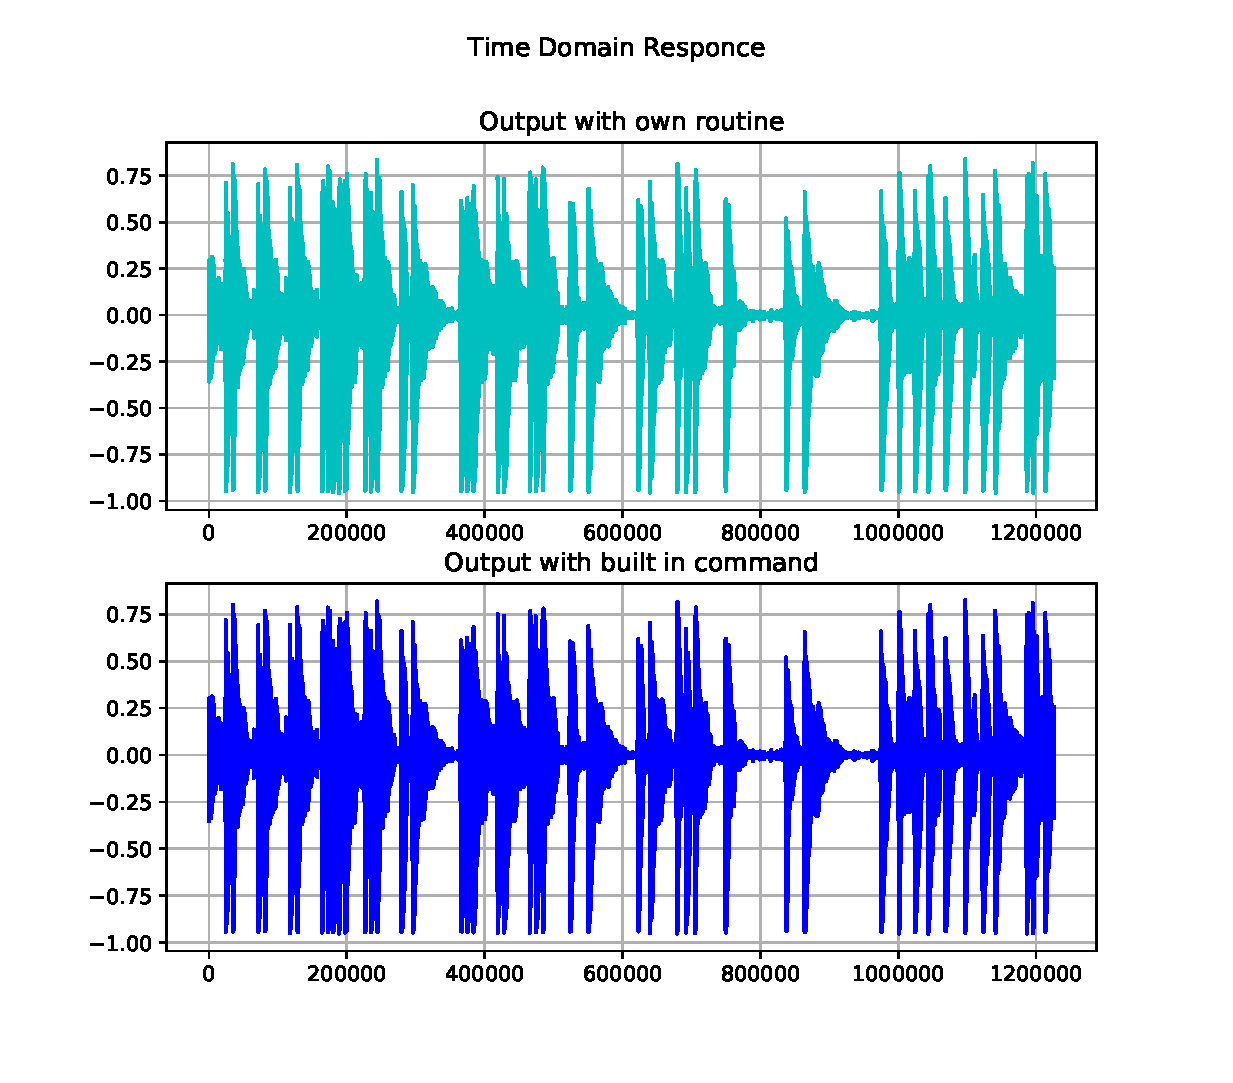
\includegraphics[width=1.2\columnwidth]{figs/ee18btech11037_1.eps}
\caption{Time domain response}
\label{fig:timeresponce}
\end{figure}
\\
Plotting the frequency domain response evaluated from both own routine and signal.filtfilt
\begin{figure}[!h]
\centering
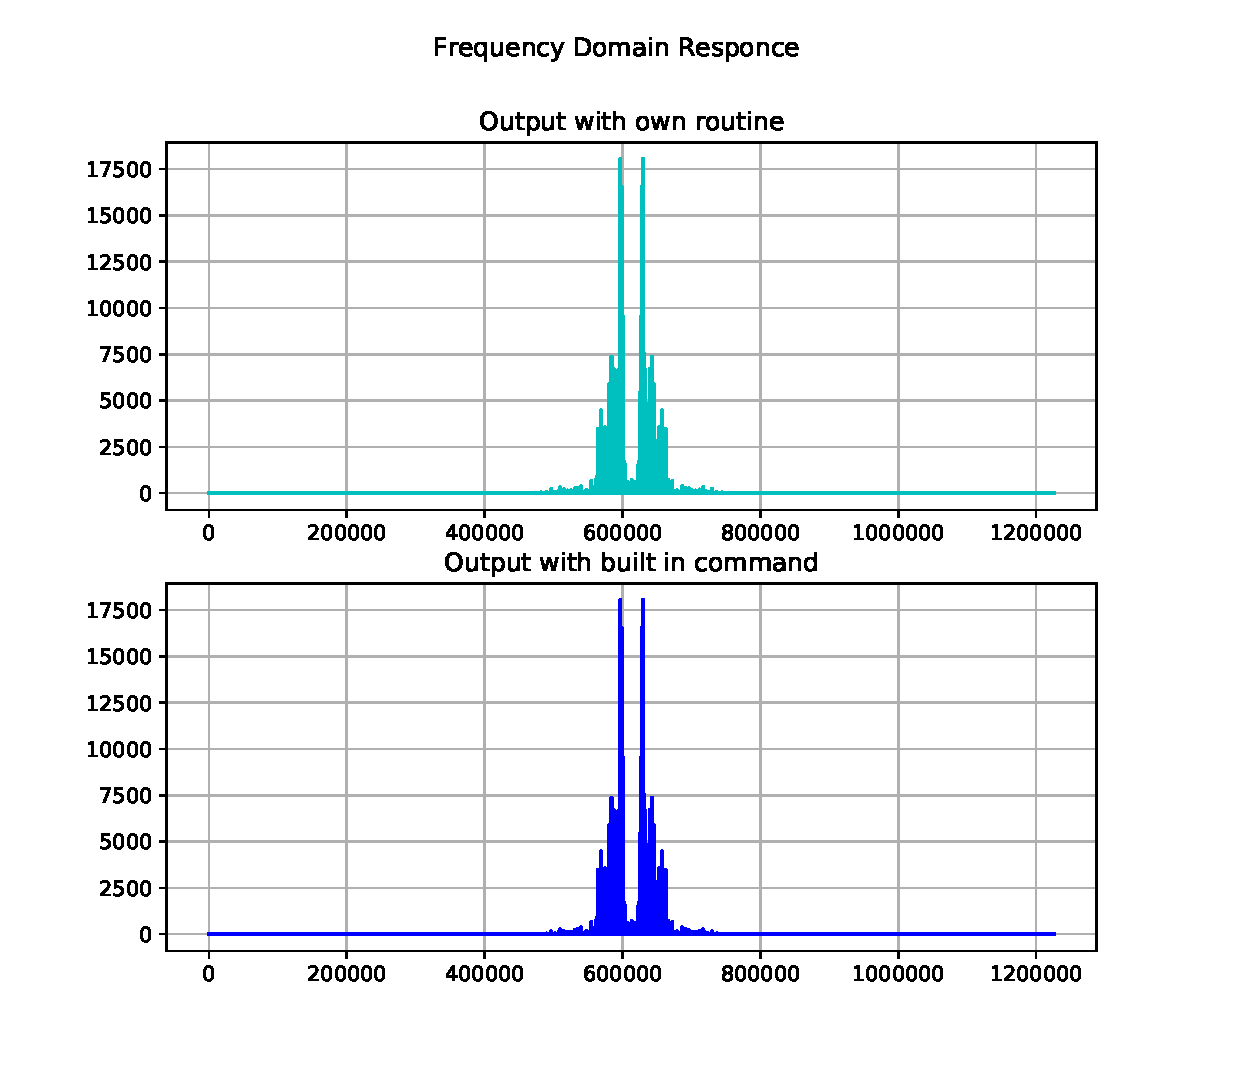
\includegraphics[width=1.2\columnwidth]{figs/ee18btech11037_2.eps}
\caption{Frequency domain response}
\label{fig:freqresponce}
\end{figure}
\end{document}